\documentclass[t]{beamer}

\subtitle{Section 2.10: The First Isomorphism Theorem}

\usepackage{amsthm,amsmath,amsfonts,hyperref,graphicx,color,multicol,soul}
\usepackage{enumitem,tikz,tikz-cd,setspace,mathtools}

%%%%%%%%%%
%Beamer Template Customization
%%%%%%%%%%
\setbeamertemplate{navigation symbols}{}
\setbeamertemplate{theorems}[ams style]
\setbeamertemplate{blocks}[rounded]

\definecolor{Blu}{RGB}{43,62,133} % UWEC Blue
\setbeamercolor{structure}{fg=Blu} % Titles

%Unnumbered footnotes:
\newcommand{\blfootnote}[1]{%
	\begingroup
	\renewcommand\thefootnote{}\footnote{#1}%
	\addtocounter{footnote}{-1}%
	\endgroup
}

%%%%%%%%%%
%TikZ Stuff
%%%%%%%%%%
\usetikzlibrary{arrows}
\usetikzlibrary{shapes.geometric}
\tikzset{
	smaller/.style={
		draw,
		regular polygon,
		regular polygon sides=3,
		fill=white,
		node distance=2cm,
		minimum height=1in,
		line width = 2pt
	}
}
\tikzset{
	smsquare/.style={
		draw,
		regular polygon,
		regular polygon sides=4,
		fill=white,
		node distance=2cm,
		minimum height=1in,
		line width = 2pt
	}
}


%%%%%%%%%%
%Custom Commands
%%%%%%%%%%

\newcommand{\C}{\mathbb{C}}
\newcommand{\quats}{\mathbb{H}}
\newcommand{\N}{\mathbb{N}}
\newcommand{\Q}{\mathbb{Q}}
\newcommand{\R}{\mathbb{R}}
\newcommand{\Z}{\mathbb{Z}}

\newcommand{\ds}{\displaystyle}

\newcommand{\fn}{\insertframenumber}

\newcommand{\id}{\operatorname{id}}
\newcommand{\im}{\operatorname{im}}
\newcommand{\Aut}{\operatorname{Aut}}
\newcommand{\Inn}{\operatorname{Inn}}

\newcommand{\blank}[1]{\underline{\hspace*{#1}}}

\newcommand{\abar}{\overline{a}}
\newcommand{\bbar}{\overline{b}}
\newcommand{\cbar}{\overline{c}}

\newcommand{\nml}{\unlhd}

%%%%%%%%%%
%Custom Theorem Environments
%%%%%%%%%%
\theoremstyle{definition}
\newtheorem{exercise}{Exercise}
\newtheorem{question}[exercise]{Question}
\newtheorem{warmup}{Warm-Up}
\newtheorem*{defn}{Definition}
\newtheorem*{exa}{Example}
\newtheorem*{disc}{Group Discussion}
\newtheorem*{nb}{Note}
\newtheorem*{recall}{Recall}
\renewcommand{\emph}[1]{{\color{blue}\texttt{#1}}}

\definecolor{Gold}{RGB}{237, 172, 26}
%Statement block
\newenvironment{statementblock}[1]{%
	\setbeamercolor{block body}{bg=Gold!20}
	\setbeamercolor{block title}{bg=Gold}
	\begin{block}{\textbf{#1.}}}{\end{block}}
\newenvironment{thm}[1]{%
	\setbeamercolor{block body}{bg=Gold!20}
	\setbeamercolor{block title}{bg=Gold}
	\begin{block}{\textbf{Theorem #1.}}}{\end{block}}


%%%%%%%%%%
%Custom Environment Wrappers
%%%%%%%%%%
\newcommand{\enumarabic}[1]{
	\begin{enumerate}[label=\textbf{\arabic*.}]
		#1
	\end{enumerate}
}
\newcommand{\enumalph}[1]{
	\begin{enumerate}[label=(\alph*)]
		#1
	\end{enumerate}
}
\newcommand{\bulletize}[1]{
	\begin{itemize}[label=$\bullet$]
		#1
	\end{itemize}
}
\newcommand{\circtize}[1]{
	\begin{itemize}[label=$\circ$]
		#1
	\end{itemize}
}
\newcommand{\slide}[1]{
	\begin{frame}{\fn}
		#1
	\end{frame}
}
\newcommand{\slidec}[1]{
\begin{frame}[c]{\fn}
	#1
\end{frame}
}
\newcommand{\slidet}[2]{
	\begin{frame}{\fn\ - #1}
		#2
	\end{frame}
}


\newcommand{\startdoc}{
		\title{Math 425: Abstract Algebra 1}
		\author{Mckenzie West}
		\date{Last Updated: \today}
		\begin{frame}
			\maketitle
		\end{frame}
}

\newcommand{\topics}[2]{
	\begin{frame}{\insertframenumber}
		\begin{block}{\textbf{Last Section.}}
			\begin{itemize}[label=--]
				#1
			\end{itemize}
		\end{block}
		\begin{block}{\textbf{This Section.}}
			\begin{itemize}[label=--]
				#2
			\end{itemize}
		\end{block}
	\end{frame}
}

\begin{document} 
	\startdoc
	
	\topics{
		\item Factor Groups
		\item Commutator Subgroups
	}{
		\item Kernels
		\item The first isomorphism theorem
	}

\slide{
	\begin{defn}
		Let $\alpha:G\to H$ be a group homomorphism.  The \emph{image of $\alpha$} is the set
			\[\im\alpha=\alpha(G)=\{\alpha(g)\ |\ g\in G\}.\]
			
		The \emph{kernel of $\alpha$} is the set
			\[\ker\alpha=\{k\in G\ |\ \alpha(k)=e_H\}.\]
	\end{defn}
	\begin{exercise}
		Let $\alpha:\Z\to \C^*$ be defined by $\alpha(n)=i^n$ where $i=\sqrt{-1}$.
		
		Compute $\ker(\alpha)$.  
	\end{exercise}
}


\slide{
	\begin{thm}{Almost 2.10.1}
		If $\alpha:G\to H$ is a group homomorphism, then $\ker\alpha$ is a subgroup of $G$.
	\end{thm}
	\begin{exercise}
		Let $\alpha:\Z\to \C^*$ be defined by $\alpha(n)=i^n$ where $i=\sqrt{-1}$.
		
		What are the cosets of $\ker(\alpha)$?
	\end{exercise}
}
%\slide{
%	\begin{block}{\textbf{Observation.}}
%		If $a\ker(\phi)=b\ker(\phi)$, then $\phi(a)=\phi(b)$!  We'll come back to this soon.
%	\end{block}
%}
\slide{
	\begin{thm}{2.10.1}
		Let $\alpha:G\to H$ be a group homomorphism.  Then
		\enumarabic{\item $\alpha(G)$ is a subgroup of $H$. \item $\ker(\alpha)$ is a \textbf{normal} subgroup of $G$}
	\end{thm}
}
\slide{
	\begin{exercise}
		\enumalph{
			\item Prove $SL_2(\R)\lhd GL_2(\R)$.\vskip 1in 
			\item Prove $A_n\lhd S_n$.
		}
	\end{exercise}
}

\slide{
	\begin{thm}{2.10.3}
		Let $\alpha:G\to H$ be a group homomorphism.  Then $\alpha$ is injective if and only if $\ker(\alpha)=\{e_G\}$.
	\end{thm}
}

\slide{
	\begin{statementblock}{The First Isomorphism Theorem (2.10.4)}
		Let $\alpha: G\to H$ be a group homomorphism. Then $$G/\ker\alpha\cong im(G)=\alpha(G).$$
	\end{statementblock}
}

\slide{
	So here we have a map $\alpha:G\to H$. Let $K=\ker(\alpha)$. 
		\vskip 2em
	Define $\overline{\alpha}: G/K\to im(\alpha)$ by $\overline{\alpha}(aK)=\alpha(a)$ for all $a\in G$.
		\vskip 2em
	Claim: $\overline{\alpha}$ is an isomorphism.
	
	\begin{nb}
		Since the domain of $\alpha$ is a quotient, we have to first make sure that $\alpha$ is well-defined. **Elements in the domain can be represented in multiple ways.**
	\end{nb}
}

\slide{
	\begin{proof}[Proof ($\overline{\alpha}$ is well-defined and one-to-one).]
		\vskip 2.5in
	\end{proof}
}
\slide{
\begin{proof}[Proof ($\overline{\alpha}$ is onto).]
	\vskip 2.5in
\end{proof}
}
\slide{
\begin{proof}[Proof ($\overline{\alpha}$ is a homomorphism)]
	\vskip 2.5in
\end{proof}
}
\slide{
	\begin{exercise}
		Prove that $\Z/n\Z\cong \Z_n$ for all integers $n\geq 1$.
	\end{exercise}
}
\begin{frame}[fragile]
	\frametitle{\fn}
	\begin{recall}
		If $a+bi\in \C$ for $a,b\in\R$, we can plot this as the point $(a,b)$.
		
		Moreover, any point on unit circle corresponds to the complex number $e^{i\theta}$ where $\theta$ is the angle between the vector defined by the point and the positive $x$-axis:
		
		\begin{center}
			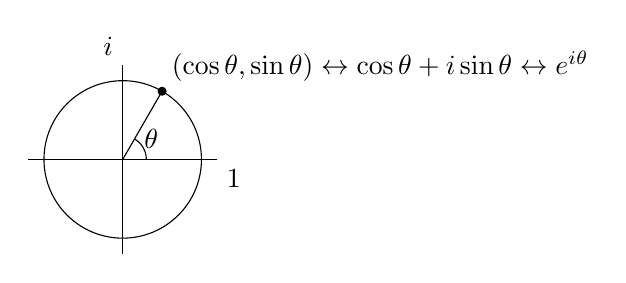
\begin{tikzpicture}
				\draw (0,0) circle (1);
				\filldraw (0,0) -- (60:1) circle (.05) node[anchor=south west] {$(\cos\theta,\sin\theta)\leftrightarrow \cos\theta+i\sin\theta\leftrightarrow e^{i\theta}$};
				\draw (.3,0) arc (0:60:.3) node[anchor=west] {$\theta$};
				\draw (-1.2,0) -- (1.2,0) node[anchor=north west] {$1$};
				\draw (0,-1.2) -- (0,1.2) node[anchor=south east] {$i$};
			\end{tikzpicture}
		\end{center}
		
		
		Claim: The unit circle,$$\C^0 = \{z\in \C:|z|=1\}=\{e^{i\theta} : 0\leq \theta < 2\pi\}=\{e^{i\theta} : \theta\in \R\}$$ is a subgroup of $\C^\times$ (operation is multiplication).
	\end{recall}
\end{frame}
\slide{
	\begin{exercise}
		Prove that $\R/\Z$ (under addition) is isomorphic to $\C^0$ (under multiplication).
	\end{exercise}
}

\slide{
	\begin{statementblock}{Claim}
		If $K_1\lhd G_1$ and $K_2\lhd G_2$, then $K_1\times K_2\lhd G_1\times G_2$ and 
		\[(G_1\times G_2)/(K_1\times K_2)\cong G_1/K_1\times G_2/K_2.\]
	\end{statementblock}
}
\slide{\begin{exercise}
		Let $D_3=\{e,r,r^2,f,fr,fr^2\}$ with $|r|=3$, $|f|=2$, and $rf=fr^3$.
		
		How many homomorphisms are there from $D_3$ to $C_6$?
		
		Hint: The only normal subgroups of $D_3$ are $\{e\}$, $\langle r\rangle=\{e,r,r^2\}$, and $D_3$.
		\vskip 1.5in\mbox{}
\end{exercise}}
\slide{
	\begin{recall}
		The \emph{inner automorphism} of the group $G$ corresponding to the element $a\in G$ is the isomorphism \[\sigma_a:G\to G\quad\text{defined by}\quad\sigma_a(g)=aga^{-1}\ \forall g\in G.\]
		
		Moreover the set of inner automorphisms, $\Inn(G)=\{\sigma_a\ |\ a\in G\}$, is a subgroup of $\Aut(G)$ because $\sigma_a\circ\sigma_b=\sigma_{ab}$.
	\end{recall}
	\begin{exercise}
		There's a natural map $\alpha: G\to \Inn (G)$ defined by $\alpha(a)=\sigma_a$ for all $a\in G$.  Prove that $\alpha$ is a homomorphism.  What does the First Isomorphism Theorem tell us?
	\end{exercise}
}
\slide{
	\begin{thm}{2.10.5}
		If $G$ is any group then $G/Z(G)\cong \Inn(G)$.
	\end{thm}
}
\slide{\begin{exercise}
		Use Theorem 2.10.5 to show that $\Inn(S_3)\cong S_3$.
		\vskip .75in
		Then show that $|\Aut(S_3)|\leq 6$. By considering the possible images of $\sigma=(1\ 2\ 3)$ and $\tau=(1\ 2)$.
		\vskip .75in
		Conclude $S_3\cong \Aut(S_3)$.
		\vskip .75in\mbox{}
\end{exercise}}
\end{document}

